% Per-Principle Pass Rates — Chapter 7
% Bar chart showing pass rates across APIs.guru dataset
% Note: Values are placeholders (marked with TODO) pending actual evaluation data
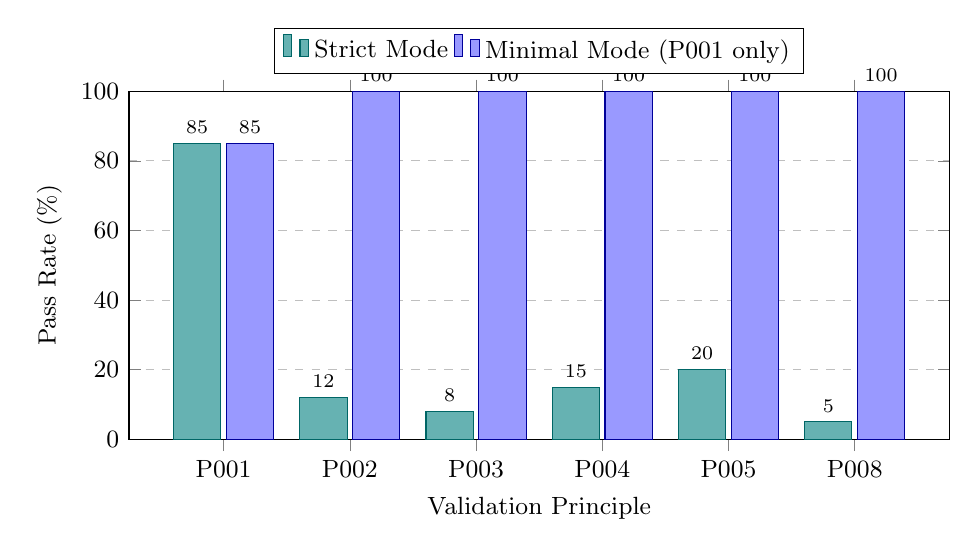
\begin{tikzpicture}
\begin{axis}[
    ybar,
    bar width=0.6cm,
    width=12cm,
    height=6cm,
    ylabel={Pass Rate (\%)},
    xlabel={Validation Principle},
    ymin=0, ymax=100,
    symbolic x coords={P001,P002,P003,P004,P005,P008},
    xtick=data,
    nodes near coords,
    nodes near coords align={vertical},
    every node near coord/.append style={font=\scriptsize},
    enlarge x limits=0.15,
    legend style={at={(0.5,1.05)},anchor=south,legend columns=2,font=\small},
    tick label style={font=\small},
    label style={font=\small},
    ymajorgrids=true,
    grid style=dashed,
]

% Strict mode pass rates (placeholder values — TODO: replace with actual data)
\addplot[fill=teal!60,draw=teal!80!black] coordinates {
    (P001,85) (P002,12) (P003,8) (P004,15) (P005,20) (P008,5)
};

% Minimal mode pass rates (placeholder values — TODO: replace with actual data)
\addplot[fill=blue!40,draw=blue!60!black] coordinates {
    (P001,85) (P002,100) (P003,100) (P004,100) (P005,100) (P008,100)
};

\legend{Strict Mode, Minimal Mode (P001 only)}

\end{axis}
\end{tikzpicture}
